\chapter{RESULT AND DISCUSSION}
\label{ch:results}

This chapter reports what the system achieves and where it fails. The dataset is described first, then the recognition results under the signer-independent protocol, then the deployment measurements, and a discussion of the remaining weaknesses.

\section{Experiment Setup}

All training and evaluation ran on an ordinary laptop with no GPU, under Python 3.11 with TensorFlow, MediaPipe, NumPy, and scikit-learn pinned to a mutually compatible set. The classifier has 192{,}007 parameters, and a single evaluation fold completes in minutes on the processor alone.

The random seed was fixed at 42 for every run. Fixing the seed by itself proved insufficient: TensorFlow's parallel processor reductions vary between runs, and on identical data this moved per-fold accuracy by as much as 2.7 percentage points. Deterministic operations were therefore enabled explicitly, so the accuracies below are reproducible from the same data and code, not one sample from a distribution of runs.

\section{Dataset Composition}
\label{sec:datasetcomposition}

The final dataset holds 840 clips, distributed exactly evenly at 120 clips in each of the seven classes. Table~\ref{tab:composition} gives the breakdown by class and signer.

\begin{table}[H]
    \centering
    \caption{Clips by class and signer in the final dataset}
    \label{tab:composition}
    \small
    \setlength{\tabcolsep}{4pt}
    \begin{tabular}{lcccccccc|c}
        \toprule
        \textbf{Class} & \textbf{s01} & \textbf{s02} & \textbf{s03} & \textbf{s04}
                       & \textbf{s05} & \textbf{s06} & \textbf{s07} & \textbf{s08} & \textbf{Total} \\
        \midrule
        building\_on\_fire & 20 & 20 & 20 & 20 & 10 & 10 & 10 & 10 & 120 \\
        call\_police       & 20 & 20 & 20 & 20 & 10 & 10 & 10 & 10 & 120 \\
        cant\_breathe      & 20 & 20 & 20 & 20 & 10 & 10 & 10 & 10 & 120 \\
        help\_danger       & 20 & 20 & 20 & 20 & 10 & 10 & 10 & 10 & 120 \\
        need\_ambulance    & 20 & 20 & 20 & 20 & 10 & 10 & 10 & 10 & 120 \\
        need\_toilet       & 20 & 20 & 20 & 20 & 10 & 10 & 10 & 10 & 120 \\
        none               & 20 & 20 & 20 & 20 &  0 & 20 & 10 & 10 & 120 \\
        \midrule
        \textbf{Total} & 140 & 140 & 140 & 140 & 60 & 80 & 70 & 70 & \textbf{840} \\
        \bottomrule
    \end{tabular}
\end{table}

\noindent The four signers who recorded 20 clips per class were team members, who could record repeatedly. The four who recorded 10 per class include the Deaf consultants and additional volunteers, whose available time was shorter. Class balance was maintained deliberately, since an imbalanced set would have let the classifier gain accuracy by favouring whichever class was most common.

The \texttt{none} row is the one exception to that pattern. Non-signing motion does not have to be performed by any particular person to be a valid negative, so the shortfall left by the signer who recorded none of it was made up by another signer rather than by relaxing the class balance. Every class still holds exactly 120 clips; only the negative class is unevenly distributed across the people who contributed it.

Eight signers is a small number, and it is the principal limitation on how much the reported accuracy can be trusted to generalise. This is discussed in Section~\ref{sec:discussion}.

\section{Sequence Length and Standardisation}

Frame counts across the 840 clips range from 30 to 217, with a median of 89.5 and a mean of 91.7. Figure~\ref{fig:seqlen} shows the distribution. The 95th percentile falls at 146 frames, which became the fixed sequence length.

\begin{figure}[H]
    \centering
    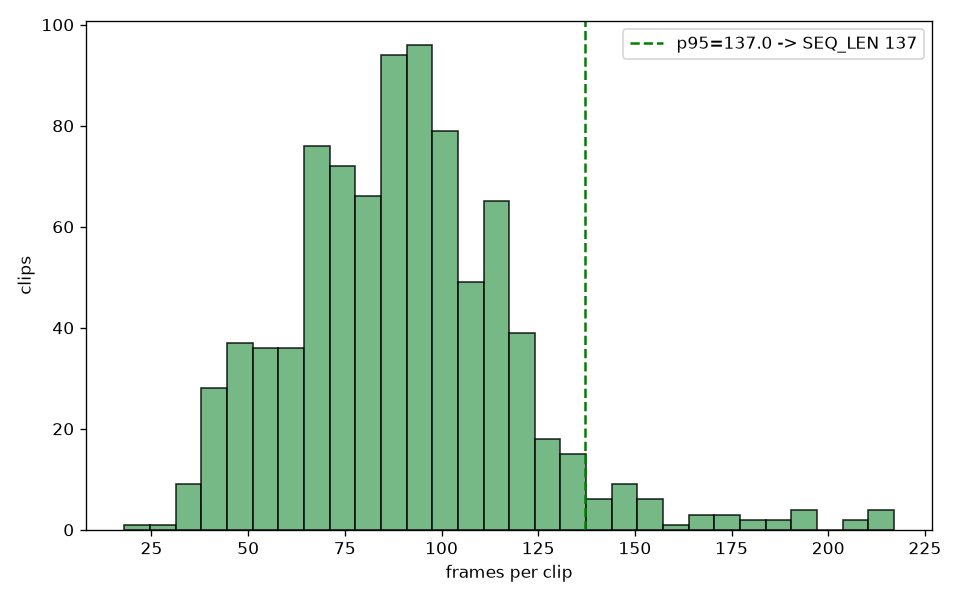
\includegraphics[width=0.75\textwidth]{img/seqlenhist.png}
    \caption{Distribution of raw clip frame counts across the 840 recorded clips, with the 95th-percentile cutoff that fixes the sequence length at 146 frames}
    \label{fig:seqlen}
\end{figure}

\noindent At a capture rate of 15.7 frames per second, 146 frames corresponds to about 9.3 seconds of signing, and the median clip of 89.5 frames to about 5.7 seconds. Table~\ref{tab:stdmodes} shows how the standardisation step treated the clips.

\begin{table}[H]
    \centering
    \caption{How the 840 clips were standardised to 146 frames}
    \label{tab:stdmodes}
    \begin{tabular}{lrp{6.4cm}}
        \toprule
        \textbf{Mode} & \textbf{Clips} & \textbf{Treatment} \\
        \midrule
        Padded ($<146$ frames)     & 794 & zero-padded at the end, with a mask recording the real frames \\
        Subsampled ($>146$ frames) & 39  & sampled at 146 evenly spaced positions \\
        Exact (146 frames)         & 7   & used unchanged \\
        \midrule
        \textbf{Total}             & \textbf{840} & \\
        \bottomrule
    \end{tabular}
\end{table}

\noindent Of the 122{,}640 frame slots in the compiled tensor, 76{,}018 hold real recorded frames and the remaining 38.0\% are zero-padding that the masking layer skips. Only 39 clips were long enough to be compressed, which matters for a reason returned to in Section~\ref{sec:discussion}: below 146 frames the model receives duration information directly in the frame count, and above it that information is normalised away.

\section{Training Behaviour}

Every fold converged and stopped on the early-stopping criterion before exhausting the 200-epoch budget. Table~\ref{tab:folds} reports where each fold stopped alongside its accuracy. The spread from 28 to 58 epochs reflects how quickly validation loss stopped improving on each training subset.

Figure~\ref{fig:curves} shows accuracy per epoch for all eight folds and Figure~\ref{fig:losscurves} the corresponding losses. Each accuracy panel carries a dashed line at that fold's held-out score. The gap between the training and validation curves, both drawn from signers inside the training set, and that dashed line is the cost of meeting a signer the model has never seen. Presenting all eight folds shows whether the folds behaved consistently, which a single representative curve cannot.

\begin{figure}[H]
    \centering
    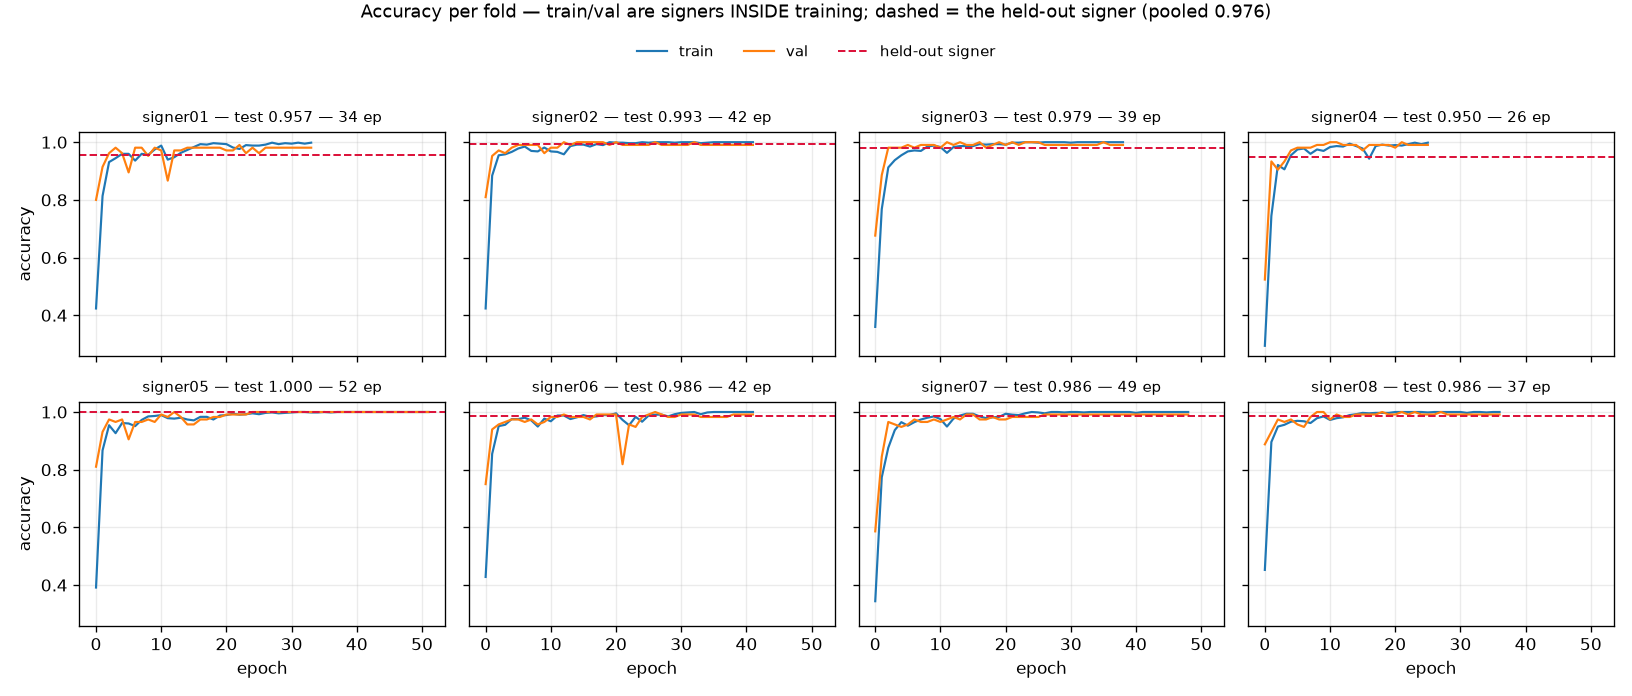
\includegraphics[width=\textwidth]{img/trainingcurves.png}
    \caption{Accuracy per epoch for each leave-one-signer-out fold. Training and validation curves are drawn from signers inside the training set; the dashed line marks the held-out signer's score.}
    \label{fig:curves}
\end{figure}

\begin{figure}[H]
    \centering
    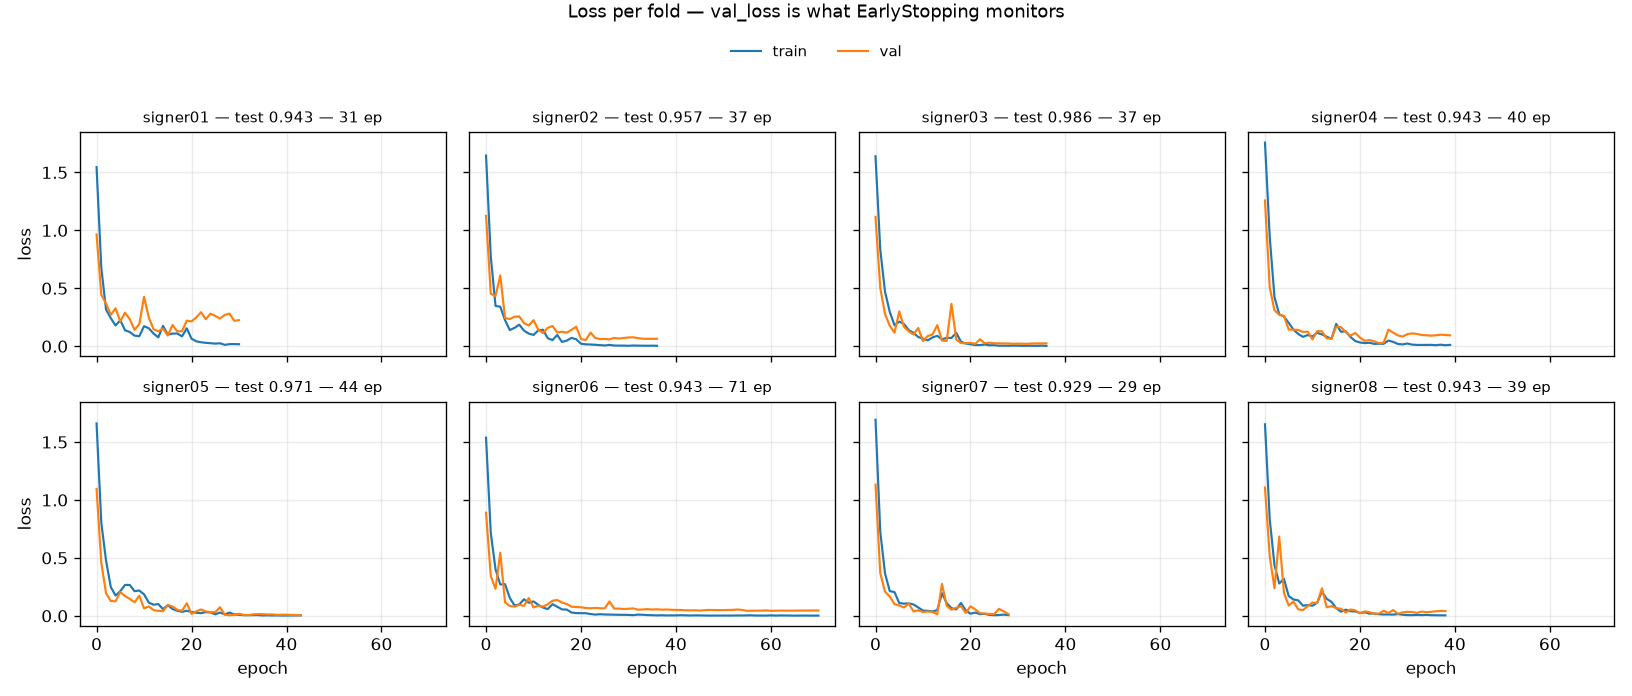
\includegraphics[width=\textwidth]{img/traininglosscurves.png}
    \caption{Loss per epoch for each fold. Validation loss is the quantity early stopping monitors.}
    \label{fig:losscurves}
\end{figure}

\section{Signer-Independent Recognition Results}

All eight signers were eligible for holdout, since removing any one of them left every class present in the remainder. Table~\ref{tab:folds} gives the result of each fold.

\begin{table}[H]
    \centering
    \caption{Leave-one-signer-out results. Each fold trains on seven signers and tests on the eighth.}
    \label{tab:folds}
    \begin{tabular}{lccc}
        \toprule
        \textbf{Held-out signer} & \textbf{Test clips} & \textbf{Accuracy} & \textbf{Epochs to stop} \\
        \midrule
        signer01 & 140 & 0.9500 & 52 \\
        signer02 & 140 & 0.9429 & 31 \\
        signer03 & 140 & 0.9786 & 40 \\
        signer04 & 140 & 0.9929 & 37 \\
        signer05 & 60  & 0.9833 & 53 \\
        signer06 & 80  & 0.9125 & 28 \\
        signer07 & 70  & 0.9714 & 58 \\
        signer08 & 70  & 0.9571 & 41 \\
        \midrule
        \multicolumn{2}{l}{\textbf{Mean across folds}}      & \textbf{0.9611} $\pm$ 0.0244 & \\
        \multicolumn{2}{l}{\textbf{Pooled over 840 clips}}  & \textbf{0.9619} & \\
        \bottomrule
    \end{tabular}
\end{table}

\noindent Mean accuracy across folds is 96.11\% with a standard deviation of 2.44 percentage points. Pooling all 840 predictions, each made by a model that had not seen its signer, gives 96.19\%.

The spread between folds is more informative than the mean. The strongest fold reaches 99.29\% and the weakest 91.25\%, a range of eight points. Since each fold differs only in which signer was withheld, that spread is a direct measurement of how much recognition quality depends on the individual. The two weakest folds are signer06 at 91.25\% and signer02 at 94.29\%, and they are not the two smallest: signer02 contributed 140 clips, the largest share in the dataset, so the difficulty is a property of how those people sign and not an artefact of a short fold in which one misclassification moves the score further. Reporting the mean alone would hide this; a system deployed to the public will meet signers at both ends of that range.

\subsection{Per-Class Performance}

Table~\ref{tab:perclass} gives precision, recall, and F1 for each class, pooled over all folds.

\begin{table}[H]
    \centering
    \caption{Per-class performance, pooled over all eight folds}
    \label{tab:perclass}
    \begin{tabular}{lcccc}
        \toprule
        \textbf{Class} & \textbf{Precision} & \textbf{Recall} & \textbf{F1} & \textbf{Support} \\
        \midrule
        \texttt{building\_on\_fire} & 0.9658 & 0.9417 & 0.9536 & 120 \\
        \texttt{call\_police}       & 0.9669 & 0.9750 & 0.9710 & 120 \\
        \texttt{cant\_breathe}      & 0.9916 & 0.9833 & 0.9874 & 120 \\
        \texttt{help\_danger}       & 0.9752 & 0.9833 & 0.9793 & 120 \\
        \texttt{need\_ambulance}    & 0.9516 & 0.9833 & 0.9672 & 120 \\
        \texttt{need\_toilet}       & 0.9917 & 0.9917 & 0.9917 & 120 \\
        \texttt{none}               & 0.8898 & 0.8750 & 0.8824 & 120 \\
        \midrule
        \textbf{Macro average}      & 0.9618 & 0.9619 & 0.9618 & 840 \\
        \bottomrule
    \end{tabular}
\end{table}

\noindent The six emergency phrases achieve F1 between 0.954 and 0.992. The negative class is clearly the weakest at 0.882, with a recall of 0.875.

That asymmetry is expected. The six phrases are each a specific, repeatable performance, and the model has 120 examples of each. The \texttt{none} class is not a phrase; it is everything else, sampled 120 times from an unbounded space of possible non-signs. No number of examples makes that category as learnable as the six, and its recall would be expected to remain the lowest even with far more data.

\subsection{Confusion Matrix}

Figure~\ref{fig:confusion} shows the pooled confusion matrix and Table~\ref{tab:confusion} the same counts numerically.

\begin{figure}[H]
    \centering
    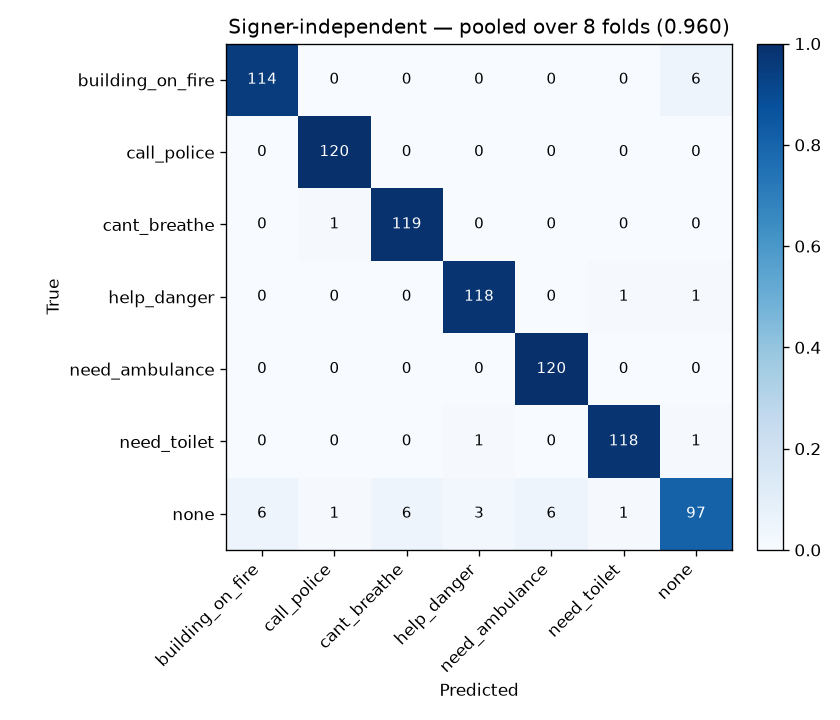
\includegraphics[width=0.8\textwidth]{img/confusionmatrix.png}
    \caption{Confusion matrix pooled over all eight leave-one-signer-out folds}
    \label{fig:confusion}
\end{figure}

\begin{table}[H]
    \centering
    \caption{Pooled confusion matrix. Rows are the true class, columns the prediction.}
    \label{tab:confusion}
    \small
    \begin{tabular}{l|ccccccc}
        \toprule
        & \rotatebox{60}{\texttt{fire}} & \rotatebox{60}{\texttt{police}} & \rotatebox{60}{\texttt{breathe}}
        & \rotatebox{60}{\texttt{help}} & \rotatebox{60}{\texttt{ambulance}} & \rotatebox{60}{\texttt{toilet}}
        & \rotatebox{60}{\texttt{none}} \\
        \midrule
        \texttt{building\_on\_fire} & \textbf{113} & 0 & 0 & 0 & 0 & 1 & 6 \\
        \texttt{call\_police}       & 0 & \textbf{117} & 0 & 0 & 0 & 0 & 3 \\
        \texttt{cant\_breathe}      & 0 & 0 & \textbf{118} & 0 & 0 & 0 & 2 \\
        \texttt{help\_danger}       & 0 & 1 & 0 & \textbf{118} & 0 & 0 & 1 \\
        \texttt{need\_ambulance}    & 1 & 0 & 0 & 0 & \textbf{118} & 0 & 1 \\
        \texttt{need\_toilet}       & 0 & 0 & 0 & 1 & 0 & \textbf{119} & 0 \\
        \texttt{none}               & 3 & 3 & 1 & 2 & 6 & 0 & \textbf{105} \\
        \bottomrule
    \end{tabular}
\end{table}

\noindent Thirty-two of the 840 predictions are wrong, and they fall into three groups that carry very different consequences.

Fifteen errors are non-signs predicted as emergency phrases, in the bottom row. These are the most serious errors the system can make, because each one is an occasion where the system would announce an emergency that nobody signed. They are spread across five of the six phrases rather than concentrated on one, which suggests a genuine resemblance between some non-signing motion and the opening of a phrase rather than a single confusable pair. \texttt{need\_ambulance} takes six of the fifteen, more than twice any other phrase, and is the one specific target this group offers.

Thirteen errors are emergency phrases predicted as \texttt{none}, in the last column, six of them for \texttt{building\_on\_fire}. Here the system stays silent when the user did sign. This leaves the user without help, though it does not produce a false alarm, and in a real deployment the user would notice the absence of a response and sign again.

Only four errors are one emergency phrase confused with another, and no pair of phrases accounts for more than a single one of them. A wrong phrase is worse than silence, because it sends the wrong help, so it is worth stating that this most damaging category is also the rarest: four occurrences in 840 predictions, none of them a repeated confusion that could be attributed to two phrases genuinely resembling each other.

The errors that remain are therefore almost entirely a question of the boundary between signing and not signing: twenty-eight of the thirty-two involve the \texttt{none} class in one direction or the other. Section~\ref{sec:weakpoint} takes that up.

\section{What the Random Split Shows}
\label{sec:leakage}

Under a stratified 70/15/15 random split, the same architecture and the same training recipe reach 99.21\% accuracy on 126 held-out clips. This is 3.0 percentage points above the signer-independent figure.

That gap is the point of reporting the number. Under a random split, clips from the same person appear in both training and test, so the model can score well by recognising the individual as much as the sign. The signer-independent protocol removes that possibility, and the accuracy falls. The 99.21\% figure describes how well the system recognises phrases performed by people it has already been trained on, which is not the situation any real user is in.

\begin{table}[H]
    \centering
    \caption{The two evaluation protocols compared}
    \label{tab:protocols}
    \begin{tabular}{lcc}
        \toprule
        \textbf{Protocol} & \textbf{Accuracy} & \textbf{What it measures} \\
        \midrule
        Random split, stratified 70/15/15 & 0.9921 & performance on known signers \\
        Signer-independent, mean of 8 folds & 0.9611 & performance on a new signer \\
        Signer-independent, pooled & 0.9619 & performance on a new signer \\
        \bottomrule
    \end{tabular}
\end{table}

\noindent This is worth stating because published NSL recognition results are generally reported without separating signers, including the closest prior landmark-based work \cite{shrestha2024nsl}. A comparison of headline accuracies across papers is therefore not meaningful unless the protocols match. On this dataset the difference between the two protocols is 3.0 points, and a project reporting only the higher number would not be doing anything unusual by the standards of the field.

\section{Generalisation and Overfitting}
\label{sec:generalisation}

A model with 192{,}007 parameters trained on 840 clips has enough capacity to memorise its
training set, so whether it has done so is a question the evaluation has to answer rather
than assume. Three accuracies are available for each fold, and the distance between them is
what the question turns on.

\begin{table}[H]
    \centering
    \caption{The three levels of accuracy, and what the gap between each pair means}
    \label{tab:threelevels}
    \small
    \begin{tabular}{|p{3.3cm}|p{4.0cm}|p{5.4cm}|}
        \hline
        \textbf{Measured on} & \textbf{Drawn from} & \textbf{A large gap to the next level means} \\
        \hline
        Training clips & signers inside training & the model is fitting its own examples \\
        \hline
        Validation clips & signers inside training, clips held out & memorisation of individual clips \\
        \hline
        Held-out signer & a person absent from training & memorisation of the people, not the signs \\
        \hline
    \end{tabular}
\end{table}

\noindent Four pieces of evidence bear on overfitting.

First, no fold ran to the epoch limit. Early stopping halted every fold between 28 and 58
epochs against a budget of 200, monitoring validation loss with the best weights restored.
A model still improving on held-out data at the point it stops has not begun to memorise;
a model that needed the full 200 epochs and kept its final weights would be the worrying
case.

Second, the regularisation is not nominal. Two dropout layers at 0.3 sit between the
recurrent layers, the learning rate halves after six epochs without improvement, and the
masking layer removes padded frames from the computation so they cannot be fitted as
signal.

Third, the per-fold spread is narrow. Eight independently trained models, each missing a
different signer, produce accuracies between 0.9125 and 0.9929 with a standard deviation
of 2.44 percentage points. A model that had memorised its training signers would be
expected to collapse on some folds and not others, giving a much wider spread than this.

Fourth, and least comfortably, the random-split comparison puts a number on the
memorisation that does remain. The 3.0-point gap between 99.21\% and 96.19\% is the
portion of a random-split score that comes from recognising people rather than phrases. It
is small, but it is not zero, and it is the reason the signer-independent figure is the one
quoted throughout this report.

Taken together these say the model generalises to a new signer with a loss of roughly three
points against a same-signer measurement, and that it is not overfitting in the
sense of having memorised its training clips. What they do not say is that it generalises
to a new signer drawn from outside the population of eight, which is a separate claim and
is addressed in Section~\ref{sec:discussion}.

\section{Architecture Comparison}
\label{sec:ablation}

The layer sizes in Table~\ref{tab:architecture} were settled before any of the accuracies
above existed, and nothing reported so far establishes that they were the right choice. The
protocol in Section~\ref{sec:archcompare} tests them: six variants of the architecture,
each evaluated over the same eight leave-one-signer-out folds with the same seed, split, and
callbacks, so that a difference between them is a property of the architecture and not of
the training regime. Table~\ref{tab:ablation} gives the result and
Figure~\ref{fig:ablation} shows the same numbers as intervals.

\begin{table}[H]
    \centering
    \caption{Architecture variants under the leave-one-signer-out protocol, ranked by mean accuracy. All six use bidirectional LSTM cells. Units are given as first recurrent layer / second recurrent layer / dense head; a dash marks a layer the variant does not have.}
    \label{tab:ablation}
    \small
    \setlength{\tabcolsep}{4pt}
    \begin{tabular}{lcccccc}
        \toprule
        \textbf{Architecture} & \textbf{Units} & \textbf{Dropout} & \textbf{Params} & \textbf{Mean} & \textbf{95\% CI} & \textbf{Epochs} \\
        \midrule
        bigger                 & 128/64/64  & 0.3 & 535{,}559 & 0.965 & [0.947, 0.983] & 43 \\
        \textbf{current}       & 64/32/32   & 0.3 & 192{,}007 & 0.961 & [0.944, 0.978] & 42 \\
        single\_layer          & 64/--/32   & 0.3 & 152{,}839 & 0.960 & [0.939, 0.980] & 43 \\
        no\_dense\_head        & 64/32/--   & 0.3 & 190{,}151 & 0.952 & [0.930, 0.974] & 40 \\
        high\_dropout          & 64/32/32   & 0.5 & 192{,}007 & 0.947 & [0.925, 0.970] & 50 \\
        smaller                & 32/16/16   & 0.3 & 77{,}063  & 0.944 & [0.911, 0.976] & 51 \\
        \bottomrule
    \end{tabular}
\end{table}

\noindent The \texttt{current} row is the shipped architecture measured through this same
sweep, and it reproduces the leave-one-signer-out result of Table~\ref{tab:folds} exactly:
0.9611 mean, 0.0244 standard deviation. The comparison below is therefore on the same
footing as the headline result and not a separate experiment reported alongside it.

No candidate is distinguishable from any other. The means span 0.944 to 0.965, but
with only eight folds the standard error on each one is between 0.9 and 1.7 percentage
points, and every confidence interval in the table overlaps every other. Even the widest
separation in the set, between the largest variant and the smallest, is 2.1 points against
a standard error of 1.9 on the difference.

\begin{figure}[H]
    \centering
    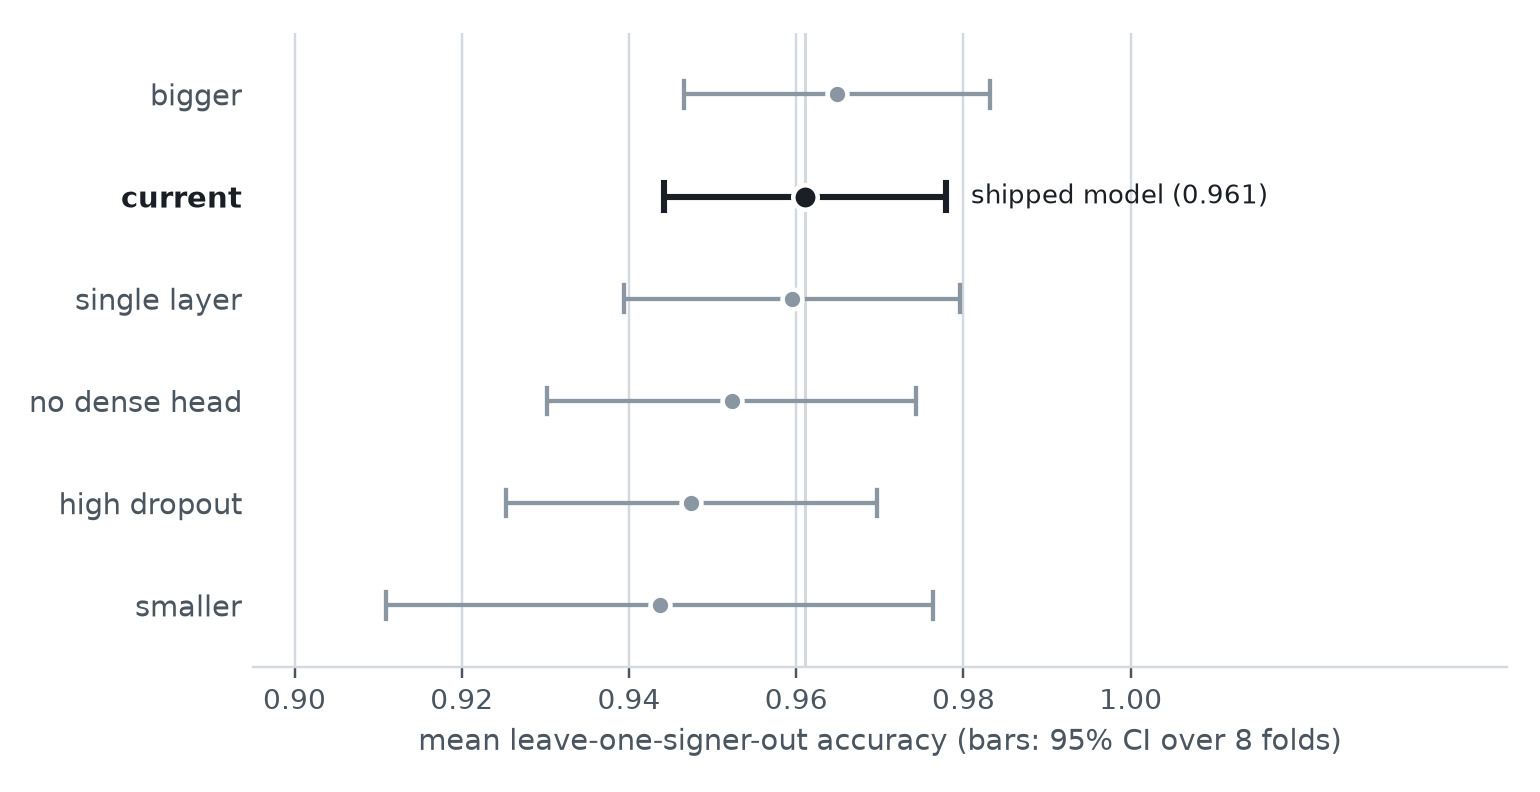
\includegraphics[width=\textwidth]{img/architecturesweep.png}
    \caption{Mean leave-one-signer-out accuracy for each architecture variant, with 95\% confidence intervals over the eight folds. The vertical rule marks the shipped model's mean; every interval crosses it.}
    \label{fig:ablation}
\end{figure}

\noindent The comparison that matters more is against the spread within each candidate. The
fold-to-fold standard deviation of a single architecture ranges from 0.024 to 0.047, which
is larger than every difference between architectures in the table. Which signer is held
out affects the result more than which architecture is trained. That is the substantive
finding of this section, and Section~\ref{sec:discussion} returns to it.

Three conclusions do follow from the table. Capacity is not the bottleneck: the largest
variant carries 535{,}559 parameters, 2.8 times the shipped model, and gains four tenths of
a point for them. A dropout rate of 0.3 is the right setting, since raising it to 0.5 is
nominally worse and needs 50 epochs to converge instead of 42. And the smallest variant is
the only one that looks genuinely handicapped --- not for its mean, which is within noise of
the rest, but for a fold-to-fold standard deviation of 0.047, nearly twice the shipped
model's, and the slowest convergence in the set. A network of 32 and 16 units is too small
to behave consistently from one held-out signer to the next.

Two properties of the comparison limit what can be read from it. Each candidate was trained
once per fold from a single seed, so run-to-run variation from weight initialisation is not
measured and could account for differences of this size by itself. And eight folds cannot
resolve differences of one or two points whatever statistical test is applied to them; that
is a property of the design and not of the analysis.

The shipped architecture is therefore retained --- not because it measurably outperforms the
alternatives, but because no alternative measurably outperforms it, and it sits at the
smaller end of the range over which accuracy has already saturated. Should the deployment
target ever impose a size budget this model misses, the single-layer variant is the one to
revisit first: dropping the second recurrent layer costs 0.16 of a percentage point, the
closest pair in the table, and removes a fifth of the parameters.

\section{Why the Accuracy Is High}
\label{sec:whyhigh}

An accuracy above 96\% on a first attempt at an under-resourced sign language invites
suspicion, and it should. Five properties of the task account for it, and three of them are
forms of optimism that a reader should discount.

The legitimate reasons come first. The problem is a seven-way choice, and the six phrases
were drawn from different semantic domains: medical, fire, crime, and basic need. Nothing
constrained them to be visually distinct, but choosing by situation produced a set whose
signed forms differ in handshape, location, and movement all at once. The confusion matrix
reflects this directly: of the twenty-one pairs of phrases that could be confused with each
other, not one is confused more than a single time in 840 predictions. Second, the landmark representation discards background, lighting, and appearance
before the model sees anything, and dual-anchor normalisation removes position and scale.
The nuisance variation that costs a pixel-based model most of its accuracy is not present
in the input. Third, the classes are exactly balanced at 120 clips each, so no part of the
score comes from favouring a common class.

The three optimistic properties matter more for interpreting the number.

Every signer reproduced a single fixed reference form, established with the consultants
before recording. This was the right methodological choice, since it fixes the ground truth
for each class, but it also means the dataset contains eight people imitating one
performance rather than eight people signing naturally. Real signing carries regional and
personal variation that this dataset largely excludes, so intra-class variance here is
lower than a deployed system would meet.

Each input is one complete phrase, performed deliberately, with the user marking its start
and end by tapping. The system never has to find a phrase inside continuous motion, decide
where one sign ends and the next begins, or handle a signer who changes their mind
mid-phrase. Segmentation is one of the harder problems in sign recognition and this design
avoids it entirely.

Half the signers are the authors, who knew the phrase set better than anyone and had the
most practice performing it. Their four folds average 0.9661 against 0.9561 for the other
four, a difference too small to be conclusive at this sample size but pointing the direction
one would expect.

None of this makes 96.19\% wrong. It makes it an accuracy on this task as specified:
seven distinct classes, one deliberate phrase at a time, performed against a fixed
reference by eight people, four of whom built the system. A wider vocabulary, natural
signing, or continuous input would each lower it.

\section{Model Export Verification}
\label{sec:exportverify}

The trained model was converted to TensorFlow Lite for deployment, reducing it from 2.3 megabytes to 881 kilobytes and removing the need for a full TensorFlow installation on the server.

A conversion fault would be indistinguishable from a model that simply performs slightly worse, so the export is verified against the original instead of trusted. Both models were run on 30 real clips and their outputs compared. The largest absolute difference in any predicted probability was $1.2 \times 10^{-7}$, and the two models agreed on the predicted class for all 30 clips. The export step refuses to write its output if this check fails.

\begin{table}[H]
    \centering
    \caption{TensorFlow Lite export verification}
    \label{tab:export}
    \begin{tabular}{lc}
        \toprule
        \textbf{Quantity} & \textbf{Value} \\
        \midrule
        Keras model size & 2.3 MB \\
        TensorFlow Lite model size & 881 KB \\
        Clips compared & 30 \\
        Largest absolute probability difference & $1.2 \times 10^{-7}$ \\
        Predicted-class agreement & 30 of 30 \\
        \bottomrule
    \end{tabular}
\end{table}

\section{Deployment}

The delivered system runs as three pieces: a container holding the server and the exported model, an Android client, and the network between them. The container omits TensorFlow entirely and runs the exported model through a lightweight runtime, which reduces the image from about three gigabytes to one.

The cost profile of a single recognition is dominated by one operation. Landmark extraction takes about 38 milliseconds per frame and accounts for almost the whole pipeline. Because frames are streamed while the user is still signing, that cost is paid concurrently with the sign, and when the client signals completion only normalisation, standardisation, and the forward pass remain, which together take about 15 milliseconds. A design that uploaded a finished recording would have serialised the two, adding several seconds of silence before every result.

\begin{table}[H]
    \centering
    \caption{Measured costs on the server path}
    \label{tab:latency}
    \begin{tabular}{lc}
        \toprule
        \textbf{Stage} & \textbf{Cost} \\
        \midrule
        Landmark extraction, per frame & $\approx$ 38 ms \\
        Normalisation, standardisation, forward pass, per clip & $\approx$ 15 ms \\
        Frames retained after decimation & 15.7 per second \\
        Client send rate cap & 16 frames per second \\
        Memory per concurrent session & $\approx$ 150 MB \\
        Concurrent session limit & 4 \\
        \bottomrule
    \end{tabular}
\end{table}

\noindent Concurrency is bounded by memory, not processor time, since each session holds its own MediaPipe graph. The session limit sheds load with an explicit error instead of allowing the process to be terminated for exhausting memory.

The Android client was built and installed on a physical device, and recognition works end to end: the user taps to begin, performs a phrase, taps to finish, and the recognised phrase appears and is spoken. End-to-end latency measured from the phone, sustained client frame rate, and per-frame encoding cost are reported in Table~\ref{tab:clientmeasurements}.

\begin{table}[H]
    \centering
    \caption{Client-side measurements on a physical device}
    \label{tab:clientmeasurements}
    \begin{tabular}{lc}
        \toprule
        \textbf{Quantity} & \textbf{Value} \\
        \midrule
        Test device & \fillin{device model} \\
        Sustained send rate while signing & \fillin{fps} \\
        Per-frame encoding cost & \fillin{ms} \\
        End-to-end latency, tap to spoken output & \fillin{seconds} \\
        \bottomrule
    \end{tabular}
\end{table}

\noindent Screenshots of the client in each of its three result states appear in Appendix~\ref{app:ui}.

\section{Development Process}

The work proceeded in seven increments, each delivering a module that could be exercised before the next began. Table~\ref{tab:sprints} records what each produced and what it changed about the plan, since several increments revised decisions made earlier.

\begin{table}[H]
    \centering
    \caption{Development increments}
    \label{tab:sprints}
    \small
    \begin{tabular}{|p{0.9cm}|p{4.2cm}|p{8.1cm}|}
        \hline
        \textbf{No.} & \textbf{Increment} & \textbf{Outcome and revisions to the plan} \\
        \hline
        1 & Consultation and phrase set & Signed form of each phrase fixed with Deaf experts. Face landmarks excluded after the consultants confirmed no phrase depends on expression. Phrase 6 changed to the toilet request. \\
        \hline
        2 & Recorder and pilot clips & Confirmed MediaPipe produces stable landmarks for multi-sign phrases. Established the zero-fill convention and the signer-encoded filename that made later signer-independent evaluation possible. \\
        \hline
        3 & Dataset collection and merge & 840 clips across 8 signers, merged through Git. The \texttt{none} class was added here, after it became clear a six-way classifier would name a phrase for any input. \\
        \hline
        4 & Preprocessing core & Sequence length derived at 146 from the measured distribution. Established that normalisation must precede padding so padded frames stay exactly zero. \\
        \hline
        5 & Training and evaluation & Leave-one-signer-out results. Two corrections came out of this stage: the early-stopping threshold had to be raised off zero, and deterministic operations had to be enabled before fold accuracies were reproducible. The architecture comparison of Section~\ref{sec:ablation} was run here, once the evaluation harness existed to run it through. \\
        \hline
        6 & Confidence thresholding & Decision rule fixed on the softmax over all seven classes, accepting a phrase only above threshold. The confidence threshold was lowered from 0.85 to 0.75 once the negative class was in place, since 0.85 was rejecting genuine signs. \\
        \hline
        7 & Export and deployment & TensorFlow Lite export with verification, inference server, and Android client. The deployment target changed from a browser to a phone at this stage, for the reasons in Section~\ref{sec:deploychange}. \\
        \hline
    \end{tabular}
\end{table}

\section{Behaviour as the Vocabulary Grows}
\label{sec:scaling}

The system recognises seven classes. Any extension of this work adds more, so it is worth
setting out what the design predicts will happen, and which parts of it break first. No
experiment in this report tests this; what follows is an argument from the structure of the
method, and it identifies where the next measurements should be taken.

\subsection{Confusion Grows Faster Than the Vocabulary}

A $K$-class problem has $K(K-1)/2$ pairs that can be confused. At seven classes there are
21, and the confusion matrix shows one of them carrying more than a single error. The
count grows quadratically: 105 pairs at fifteen classes, 435 at thirty.

The more important effect is not the arithmetic but which pairs get added. The six phrases
here were chosen by situation, not by appearance, and they happened to differ in handshape,
location, and movement simultaneously. A vocabulary of thirty NSL phrases cannot be chosen
that way. It must include pairs that differ in one parameter only, which is what
sign-language phonology calls a minimal pair, and those are exactly the cases a
146-frame landmark sequence at 15.7 frames per second is least able to separate. Two signs
distinguished by a brief change in handshape occupy a handful of frames out of 146.

The exclusion of facial landmarks becomes a limitation at this point rather than a
simplification. The consultants confirmed that none of the six current phrases depends on
facial expression, and that confirmation does not extend to a larger set. NSL, like other
sign languages, carries grammatical information on the face, including negation and
question marking. A vocabulary that includes a phrase and its negation cannot be separated
by the current 225-value feature vector at all, because the information that distinguishes
them is discarded before the model sees the input.

\subsection{The Data Requirement Scales With Classes, Not Total Clips}

What governs recognition quality is clips per class, not clips overall. Holding the present
120 per class, a thirty-class vocabulary needs 3{,}600 clips, and each new class needs its
own consultation to establish its signed form before recording can begin. The consultation
step, not the recording, is the binding constraint: it requires expert time from a small
community.

\subsection{The Negative Class Gets Harder}

The \texttt{none} class is already the weakest at 0.882 F1, and it degrades as the
vocabulary grows for a structural reason. Its job is to cover everything that is not one of
the known phrases. As known phrases multiply, the boundary between the known region and
everything else becomes longer and more intricate, while the number of \texttt{none} clips
available to describe it stays fixed. A negative class of 120 clips describing the
complement of six phrases is thin; describing the complement of thirty is thinner.

\subsection{The Confidence Threshold Needs Recalibrating}

The threshold of 0.75 requires the model to place three quarters of its probability mass on
one class. Softmax spreads probability across whatever the model finds plausible, so as
near-neighbours multiply the maximum probability falls even when the top prediction is
correct. A fixed 0.75 would therefore reject an increasing share of correct recognitions as
\texttt{low\_confidence}. The threshold is a function of vocabulary size and would have to
be recalibrated on validation data at each vocabulary, not carried forward.

\subsection{Predicted Shape of the Degradation}

Table~\ref{tab:scaling} collects these effects.

\begin{table}[H]
    \centering
    \caption{Predicted effect of a larger vocabulary on each component}
    \label{tab:scaling}
    \small
    \begin{tabular}{|p{3.5cm}|p{4.3cm}|p{4.9cm}|}
        \hline
        \textbf{Component} & \textbf{Effect of raising $K$} & \textbf{What would be needed} \\
        \hline
        Phrase classifier & Confusable pairs grow as $K^2$; minimal pairs enter the set & Higher frame rate, or explicit handshape features \\
        \hline
        Feature vector & Face-dependent distinctions become unrepresentable & Add the face block, at roughly sevenfold the input width \\
        \hline
        Training data & 120 clips per new class, plus one consultation each & Expert time, the scarcest input \\
        \hline
        \texttt{none} class & Describes a larger complement with the same clip count & Negative clips scaled with $K$ \\
        \hline
        Confidence threshold & Correct predictions fall below a fixed 0.75 & Recalibration per vocabulary size \\
        \hline
    \end{tabular}
\end{table}

\noindent The expected trajectory is therefore not a steady decline. Adding phrases that are
semantically and visually distinct from the existing six should cost little, because the
representation already separates such phrases well. Accuracy should fall sharply at the
point where the vocabulary first admits a minimal pair, and again where it admits a
face-dependent distinction, since the second of those is not a matter of degree but of
information the input does not contain.

The cheapest way to test this is to add three or four phrases chosen to be deliberately
similar to existing ones and re-run the leave-one-signer-out evaluation. That measures the
first of the two cliffs directly, at a cost of one consultation and a few hundred clips.

\section{Discussion}
\label{sec:discussion}

\subsection{What the Results Support}

Under a protocol that tests only on unseen signers, the system recognises the six emergency phrases with a pooled accuracy of 96.19\% and per-class F1 between 0.954 and 0.992. The landmark representation is what makes this achievable from 840 clips: a pixel-based model on the same data would have far more parameters to fit and far less invariance to the rooms and lighting the clips were recorded in.

The evaluation protocol is the part of this work most worth carrying forward. The 3.0-point gap between the random split and the signer-independent folds is a concrete measurement of how much a random split flatters a model on this kind of data, and it was obtained on a dataset small enough that the effect could easily have been dismissed as noise.

\subsection{Eight Signers Is the Binding Limitation}

Every accuracy in this chapter rests on eight people, four of whom are the authors. The standard deviation across folds is 2.44 points and the range is eight, which means the estimate of performance on a new signer is itself uncertain. A ninth signer with an unusual signing style could plausibly score below any fold reported here.

The architecture comparison in Section~\ref{sec:ablation} puts this on a firmer footing than an assertion. Across six architectures spanning 77{,}063 to 535{,}559 parameters, no variant is distinguishable from any other, and the fold-to-fold spread within each one is larger than every difference between them. What limits this system is not the model that was chosen but the number of people it has been measured on.

Four of the eight signers are also not fluent NSL users. They learned each phrase from the consultants' reference and reproduced it. The dataset therefore contains a mixture of fluent and learned performances, and the accuracy above is an accuracy on that mixture, not on fluent signing.

\subsection{The Negative Class Is the Weak Point}
\label{sec:weakpoint}

The \texttt{none} class carries a recall of 0.875, the lowest of the seven, and fifteen non-signs were predicted as emergency phrases. In deployment these are the errors that produce a false announcement, which is the most serious failure mode this system can have. Six of the fifteen were read as \texttt{need\_ambulance}, more than twice as many as any other phrase attracted, so the negative class fails unevenly rather than uniformly.

The errors run in both directions. Thirteen genuine phrases were assigned to \texttt{none} and would have been met with silence. Together the two directions account for twenty-eight of the thirty-two errors in the whole evaluation, which places the boundary between signing and not signing, rather than any confusion among the six phrases, at the centre of what remains to be improved.

Reducing this error is a question of what the negative class covers rather than of the threshold it is checked against. \fillin{re-check against the new run: did all fifteen clear the 0.75 confidence threshold?} Widening the \texttt{none} class with more varied non-signing motion, particularly motion resembling the opening of \texttt{need\_ambulance}, is the direct way to give the classifier a better boundary to place, and it is the single most useful addition to this evaluation.

\subsection{Duration Is Only Encoded Below the Sequence Length}

The model has no explicit time axis and reads frame count as duration, which is why the server discards frames down to the capture rate of the training data. That reasoning holds for clips shorter than 146 frames, which is 794 of the 840. For the 39 longer clips, uniform subsampling compresses the performance to look exactly 146 frames long, so their duration information is removed. Anything longer than about 9.3 seconds of signing is therefore scale-normalised and not measured. This is an acceptable engineering choice at this vocabulary size, and it would need revisiting for longer phrases.

A related effect follows from the masking layer. A frame in which MediaPipe detected neither the pose nor either hand is all zeros, and is therefore indistinguishable from padding and skipped. A clip containing many undetected frames is consequently shorter, from the model's point of view, than its frame count suggests.

\subsection{The Network Dependency}

Recognition runs on the server, so the delivered system does not work without a network connection. For a tool intended for emergencies this is a real weakness and not a neutral trade, and it is the first item in the future work of Chapter~\ref{ch:conclusion}. The reason it was accepted is given in Section~\ref{sec:deploychange}: the alternative was to reimplement the feature pipeline against a different landmark source, where a numerical mismatch produces confident wrong answers rather than an error, and the project had no measurement establishing that the two sources agree.
